\section{Results}
\subsection{Measurements for spring constant}
    From the raw spring length measurement data in Table \ref{spring}, we obtain the change amount of the spring length by $\Delta_{L_i}=L_i-L_0$ in Table \ref{spring*}.

    Since the acceleration due to gravity is exactly $9.794m/s^2$, we obtain the weights of weight stacks from their masses, as shown in Table \ref{weight}.\\
    
    \begin{table}[htbp]
        \centering
        \begin{tabular}{|c|c|c|c|c|c|}
            \hline
            \multicolumn{6}{|c|}{Unit: $[\times 10^{-2}m]\pm 0.01[\times 10^{-2}m]$}\\ \hline
            No. & spring 1 & No. & spring 2 & No. & series\\ \hline
            $L_0$ & 2.25 & $L_0$ & 2.84 & $L_0$ & 5.06\\ \hline
            $L_1$ & 4.40 & $L_1$ & 4.96	& $L_1$ & 9.25\\ \hline
            $L_2$ & 6.56 & $L_2$ & 7.08 & $L_2$ & 13.38\\ \hline
            $L_3$ & 8.70 & $L_3$ & 9.18	& $L_3$ & 17.60\\ \hline
            $L_4$ & 10.78 & $L_4$ & 11.25 & $L_4$ & 21.98\\ \hline
            $L_5$ & 12.85 & $L_5$ & 13.30 & $L_5$ & 26.09\\ \hline
            $L_6$ & 15.03 & $L_6$ &	15.42 & $L_6$ &	30.31\\ \hline
        \end{tabular}
        \caption{Spring constant measurement data}\label{spring}
    \end{table}
    \begin{table}[htbp]
        \centering
        \begin{tabular}{|c|c|c|c|c|c|}
            \hline
            \multicolumn{6}{|c|}{Unit: $[\times 10^{-2}m]\pm 0.01[\times 10^{-2}m]$}\\ \hline
            No. & spring 1 & No. & spring 2 & No. & series\\ \hline
            $\Delta_{L_1}$ & 2.15 & $\Delta_{L_1}$ & 2.12 & $\Delta_{L_1}$ & 4.19\\ \hline
            $\Delta_{L_2}$ & 4.31 & $\Delta_{L_2}$ & 4.24 & $\Delta_{L_2}$ & 8.32\\ \hline
            $\Delta_{L_3}$ & 6.45 & $\Delta_{L_3}$ & 6.34 & $\Delta_{L_3}$ & 12.54\\ \hline
            $\Delta_{L_4}$ & 8.53 & $\Delta_{L_4}$ & 8.41 & $\Delta_{L_4}$ & 16.92\\ \hline
            $\Delta_{L_5}$ & 10.60 & $\Delta_{L_5}$ & 10.46 & $\Delta_{L_5}$ & 21.03\\ \hline
            $\Delta_{L_6}$ & 12.78 & $\Delta_{L_6}$ & 12.58 & $\Delta_{L_6}$ & 25.25\\ \hline
        \end{tabular}
        \caption{Calculated spring measurement data}\label{spring*}
    \end{table}
    \begin{table}[htbp]
        \centering
        \begin{tabular}{|c|c|c|}
            \hline
            & $m[\times 10^{-3}kg]\pm 0.01[\times 10^{-3}kg]$ & $W[\times 10^{-3}N]\pm 0.01[\times 10^{-3}N]$\\ \hline
            1 & 4.83 & 47.3\\ \hline
            2 & 9.65 & 94.5\\ \hline
            3 & 14.50 & 142.0\\ \hline
            4 & 19.24 & 188.4\\ \hline
            5 & 23.99 & 235.0\\ \hline
            6 & 28.80 & 282.1\\ \hline            
        \end{tabular}
        \caption{Weight measurement data}\label{weight}
    \end{table}
    We have known that the relation between the elastic force and the change of spring length is linear. Therefore, applying the least-squares method, we can calculate the most optimal estimate of the slope and intercept of the regression line. The errorbars of $W$ and $\Delta_L$ are based on their own combined uncertainties, which is just their type $B$ uncertainties $\Delta_B$ in this case.\\
    \begin{figure}[h]    
        \begin{minipage}{0.5\linewidth}
            \[
            \begin{split}
                k_1&=\frac{\overline{\Delta_LW}-\overline{\Delta_L}\cdot\overline{W}}{\overline{\Delta_L^2}-\overline{\Delta_L}^2}\\[0.2cm]
                &\approx \frac{1.52\times10^{-2}-7.47\times10^{-2}\times0.165}{68.9\times10^{-4}-55.8\times10^{-4}}\\[0.2cm]
                &=2.22\pm 0.02kg/s^2,\\[0.4cm]
                b_1&=\overline{W}-k_1\overline{\Delta_L}\\[0.2cm]
                &\approx 0.1649\times 2.22 \times 0.07470\\[0.2cm]
                &=(-6.25\pm 12.5)\times10^{-4}N.
            \end{split}
            \]
        \end{minipage}
        \begin{minipage}{0.4\linewidth}
            \centering
            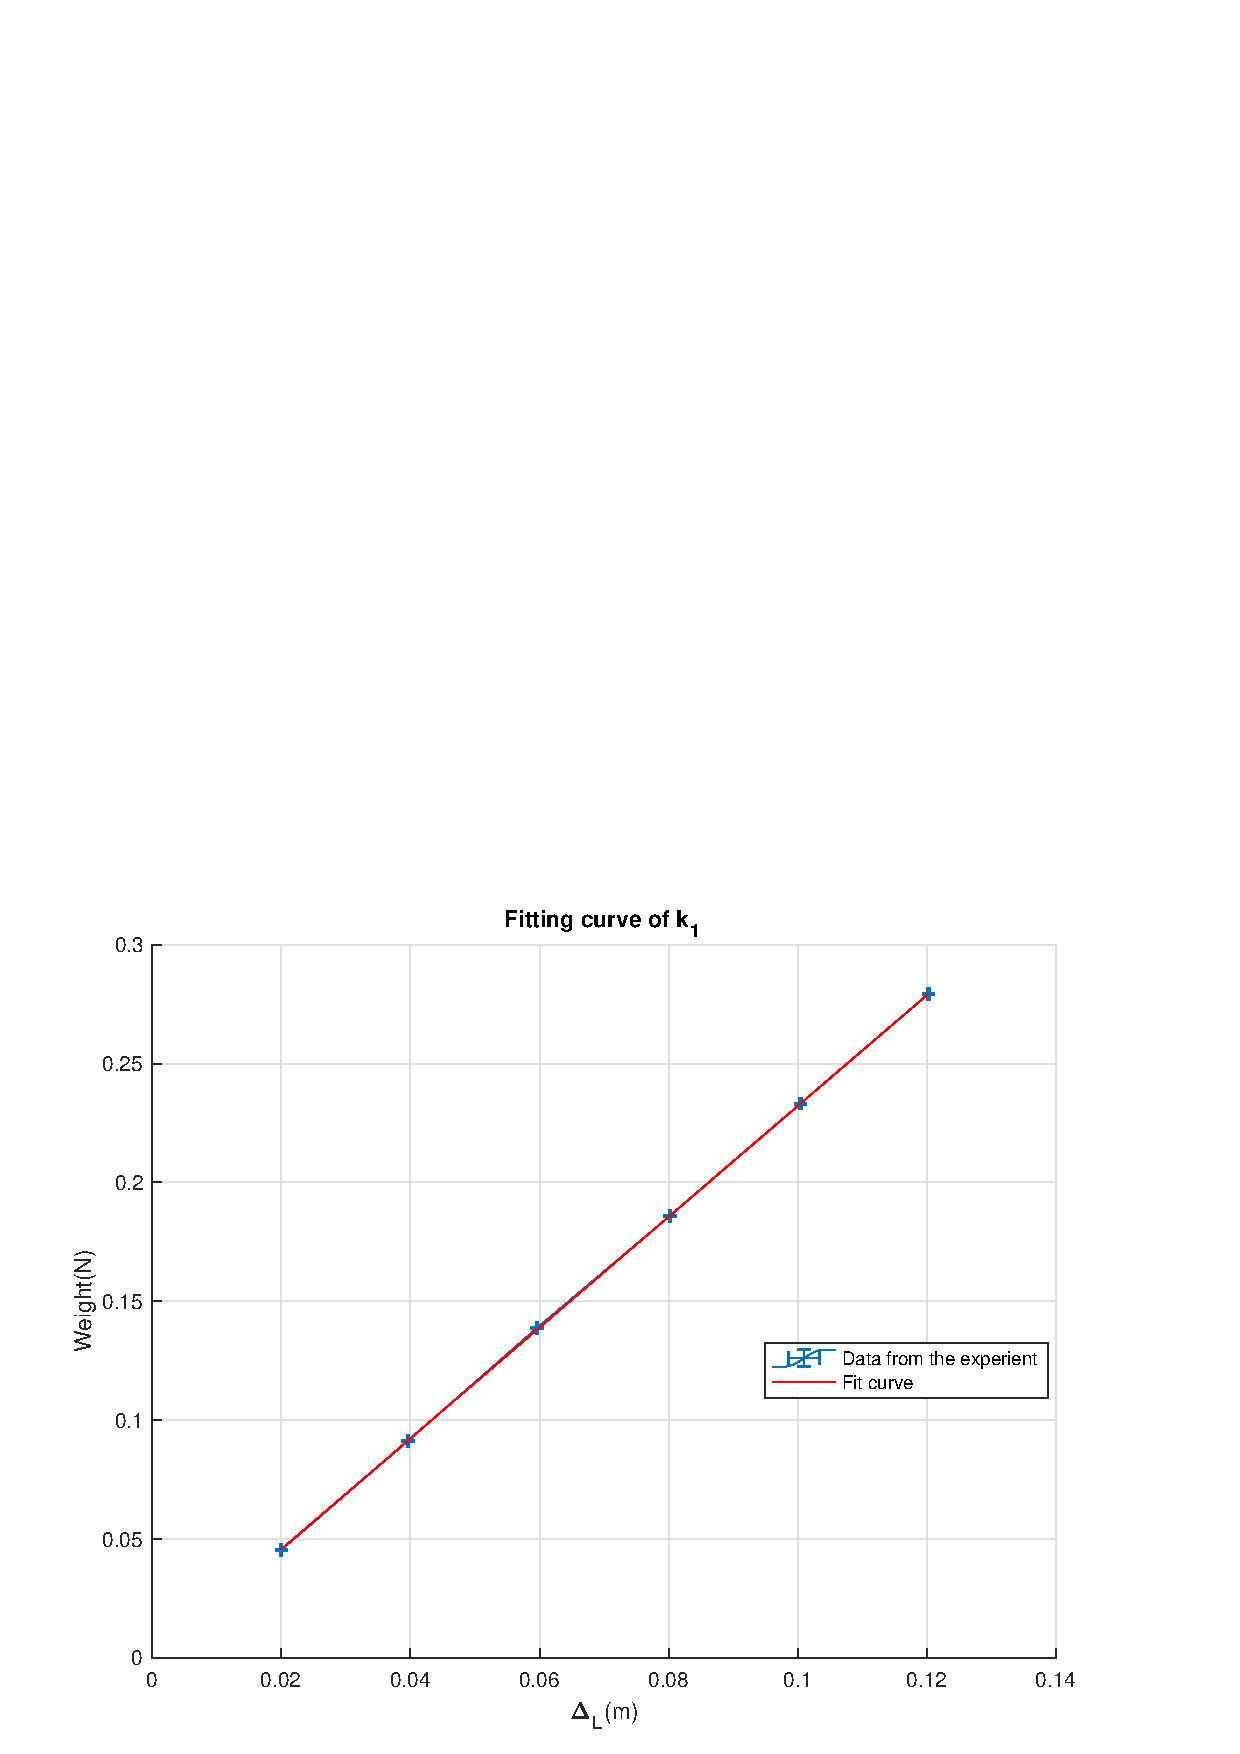
\includegraphics[height=6cm]{images/k1.png}
        \end{minipage}
        \caption{Fitting curve of spring 1}\label{k_1}
    \end{figure}

    Simliarly, we obtain $k_2$ and $k_3$.
    \[
    \begin{split}
        k_2&\approx 2.25\pm 0.01kg/s^2,\\
        b_2&\approx (-5.44\pm 70) \times10^{-4}N.
    \end{split}
    \]
    \begin{figure}[h]
        \centering
        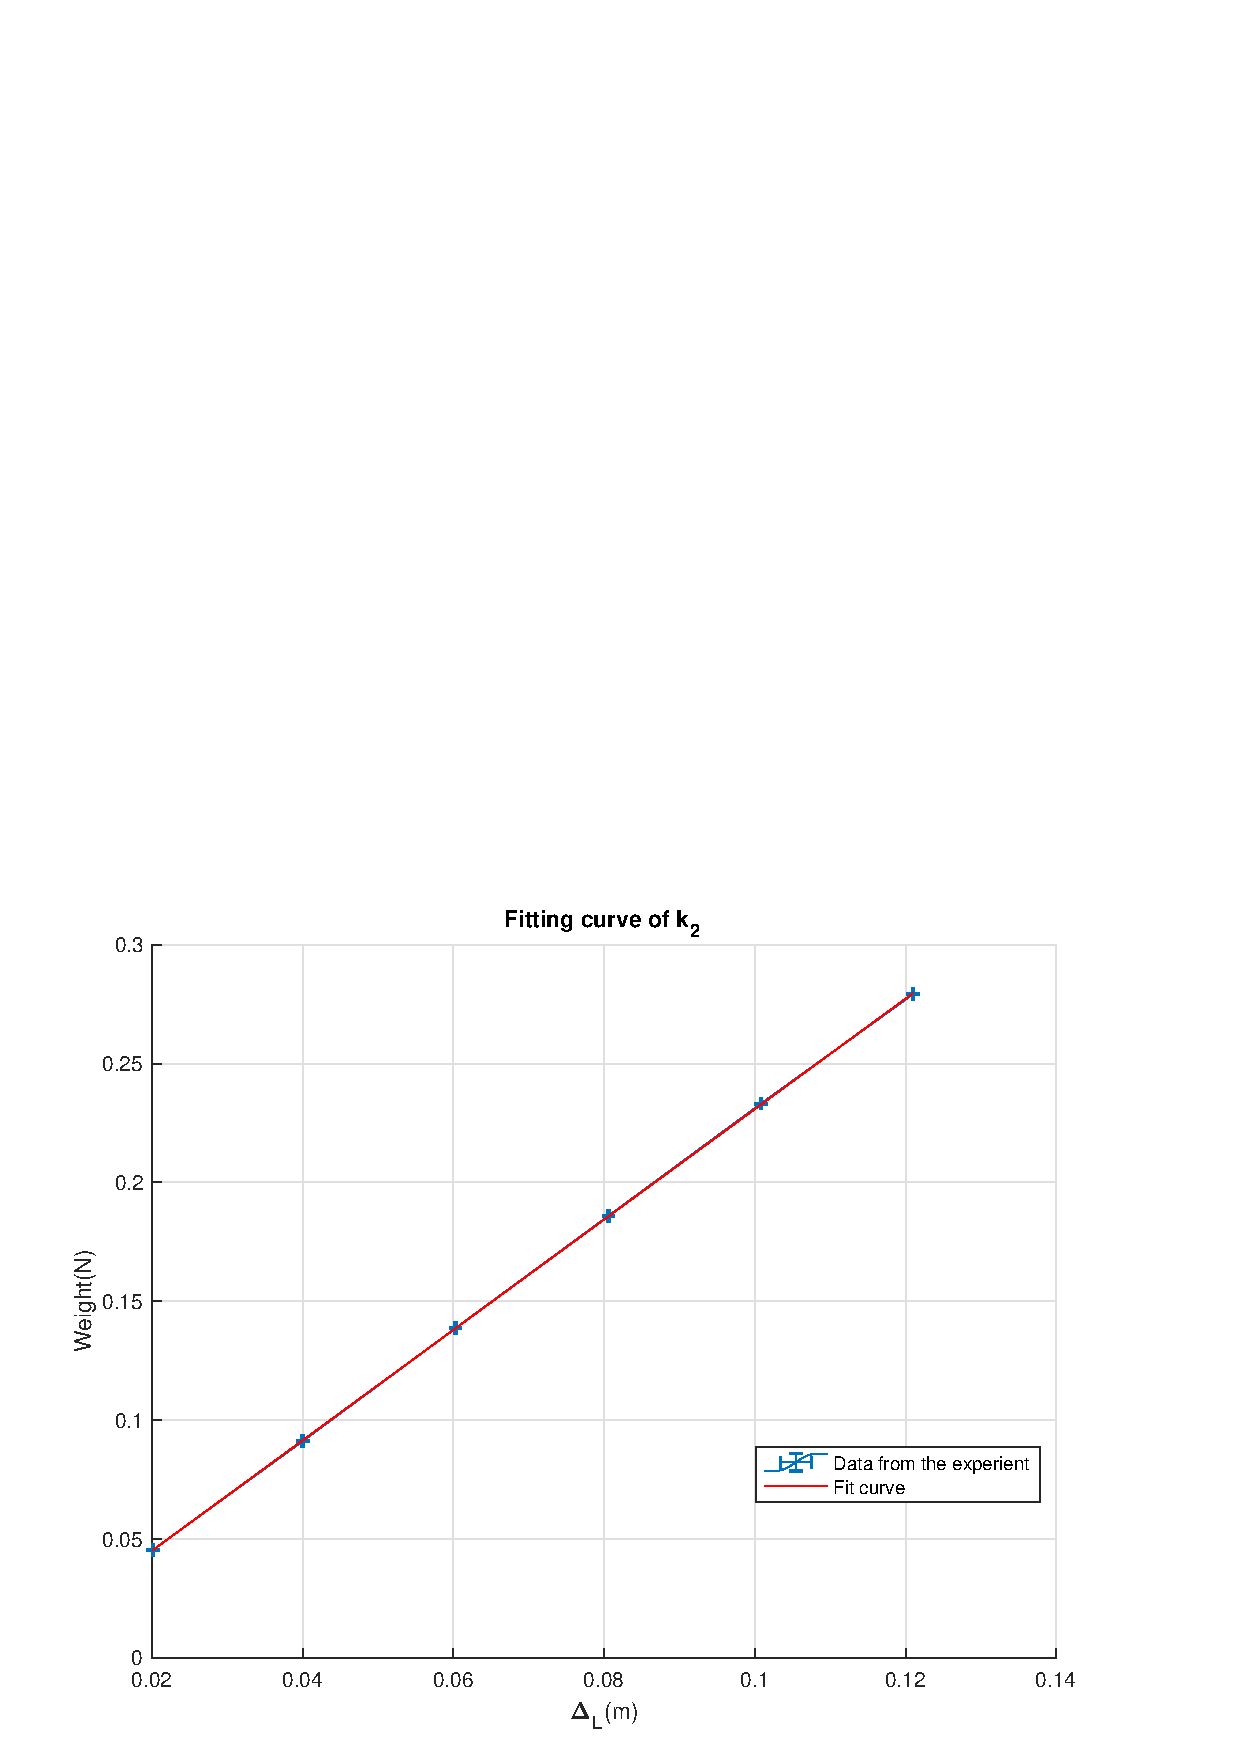
\includegraphics[height=6cm]{images/k2.png}
        \caption{Fitting curve of spring 2}\label{k_2}
    \end{figure}\\
    
    \[
    \begin{split}
        k_3&\approx 1.11\pm 0.017kg/s^2,\\
        b_3&\approx (15.1\pm 20)\times10^{-4}N.        
    \end{split}
    \]
    \begin{figure}[h]
        \centering    
        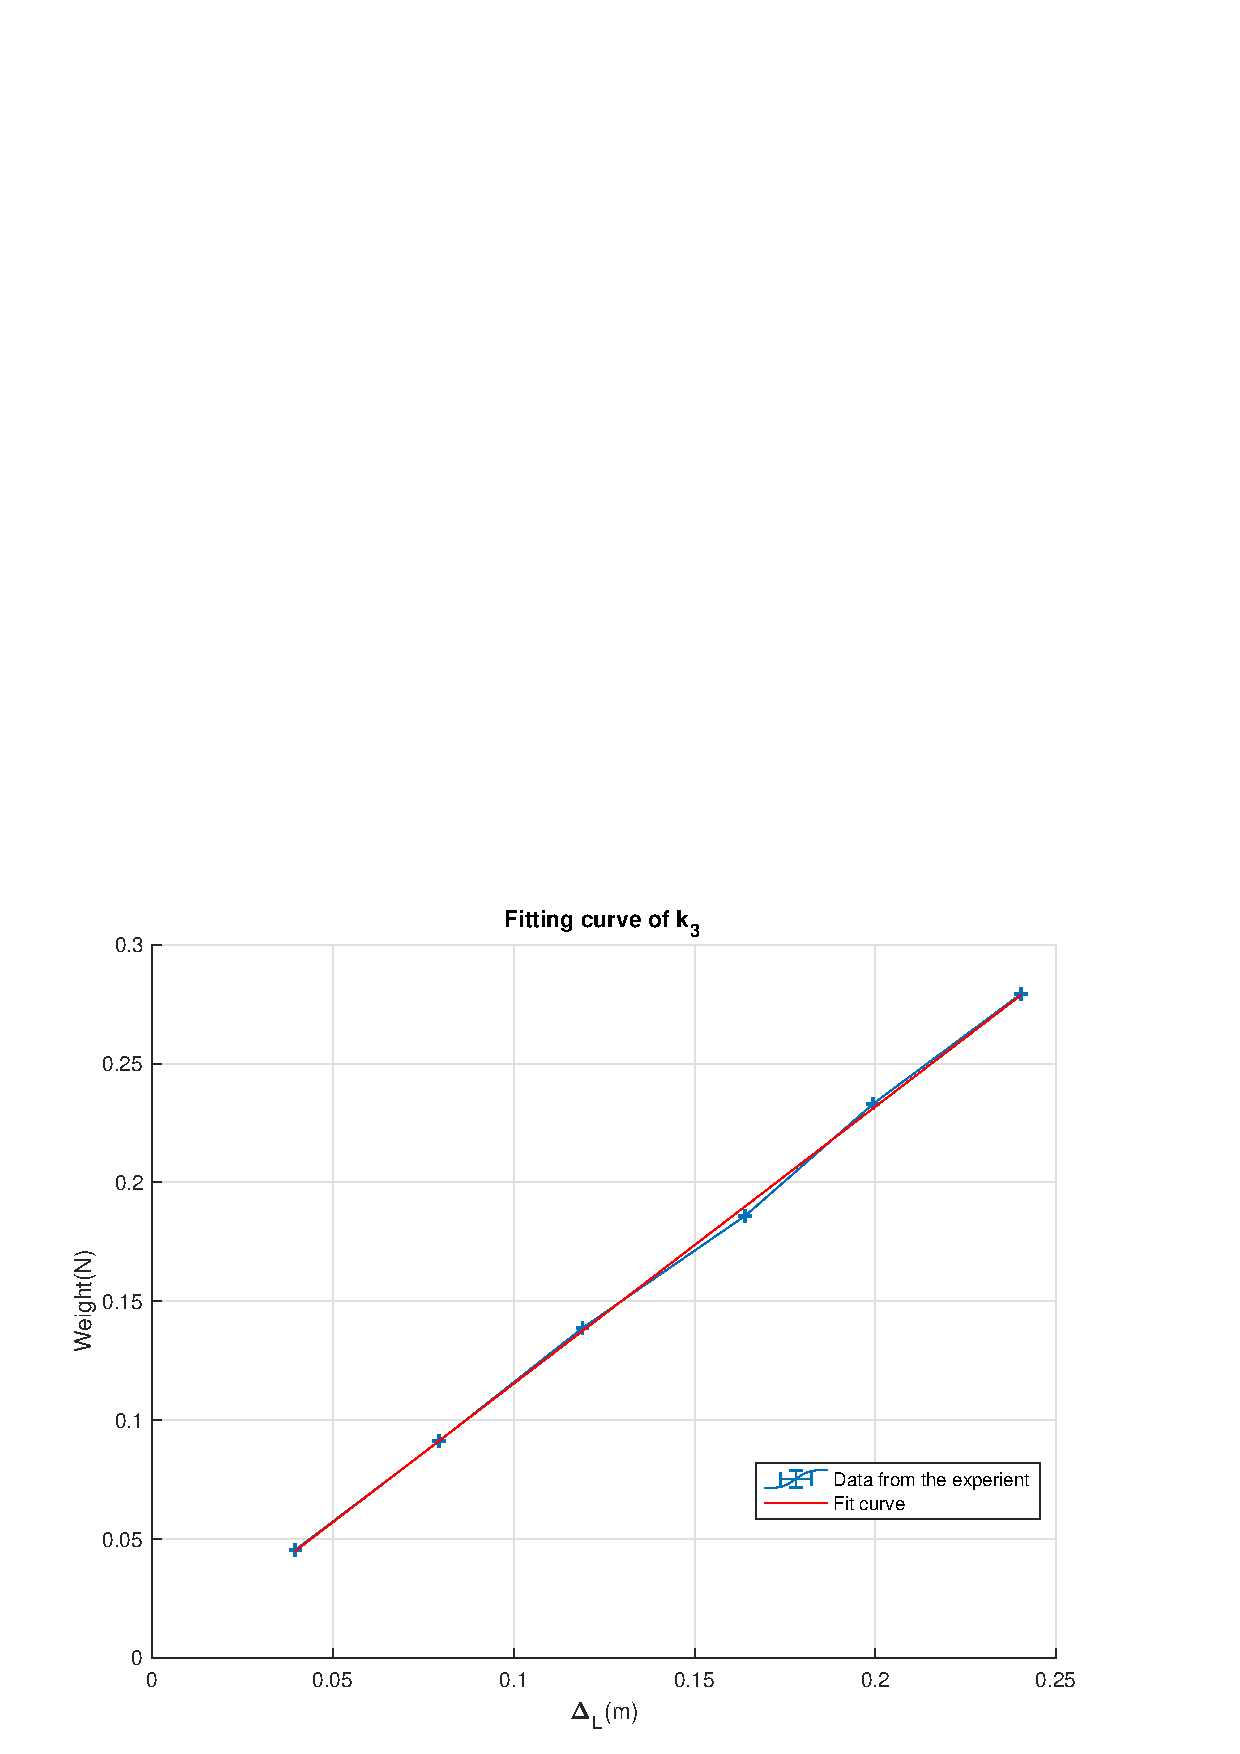
\includegraphics[height=7cm]{images/k3.png}
        \caption{Fitting curve of series of spring 1 and spring 2}\label{k_3}
    \end{figure}

    However, $k_3$ could be theoretically calculated by $k_1$ and $k_2$, which will be discussed in the section 5.\\



